\chapter{DESARROLLO}

Este capítulo detalla el proceso de diseño, construcción e implementación de la aplicación web \textit{QuickTable} para la gestión de comandas y su respectivo módulo de seguridad por hardware. El desarrollo se ejecutó siguiendo las fases metodológicas planteadas, abarcando desde la definición de requerimientos hasta las pruebas finales del sistema.

\section{Levantamiento y Especificación de Requerimientos}

De acuerdo con la metodología establecida, la primera fase del desarrollo consistió en la especificación formal de los requerimientos del software. Para garantizar la trazabilidad y la calidad en el diseño, se tomó como marco de referencia el estándar ISO/IEC/IEEE 29148 \cite{ISO29148:2018}, el cual proporciona lineamientos para la ingeniería de requerimientos en sistemas de software.

Se definieron requerimientos orientados a solucionar las problemáticas operativas, sanitarias y de seguridad informática identificadas en el sector gastronómico. A partir de la arquitectura cliente-servidor propuesta, se establecieron roles específicos para garantizar el principio del menor privilegio y segmentar las responsabilidades del negocio.


\subsection{Casos de Uso y Roles del Sistema}

El sistema fue diseñado para soportar múltiples actores operando de manera concurrente en una red local (intranet). Se definieron cinco roles principales, los cuales interactúan de forma diferenciada con el sistema:

\begin{itemize}
	\item \textbf{Administrador:} Encargado de gestionar el menú, los empleados, las mesas y visualizar reportes de ventas. Tiene acceso completo al sistema mediante validación de doble factor (2FA).
	\item \textbf{TI (Tecnología de la Información):} Rol con privilegios exclusivos para la gestión de seguridad, como la encriptación de la base de datos y la asignación de llaves físicas (NFC) a los administradores.
	\item \textbf{Mesero:} Responsable de la creación de nuevas comandas, adición de productos a pedidos existentes y visualización del estado de preparación de los platos.
	\item \textbf{Cocina:} Rol operativo que visualiza en tiempo real los pedidos entrantes y actualiza su estado (Pendiente, En Preparación, Listo).
	\item \textbf{Caja:} Encargado de procesar la facturación de las comandas consolidadas, liberar las mesas y cerrar el ciclo de venta.
\end{itemize}

Debido a la cantidad de actores y funcionalidades involucradas, el diagrama general de casos de uso se descompuso en tres vistas complementarias: autenticación y asistencia, operación diaria y administración del sistema. Cada una de estas vistas agrupa los casos de uso según el tipo de interacción y el área funcional del restaurante, lo que facilita su lectura y trazabilidad respecto a los módulos implementados en la aplicación web.

\begin{figure}[H]
	\centering
	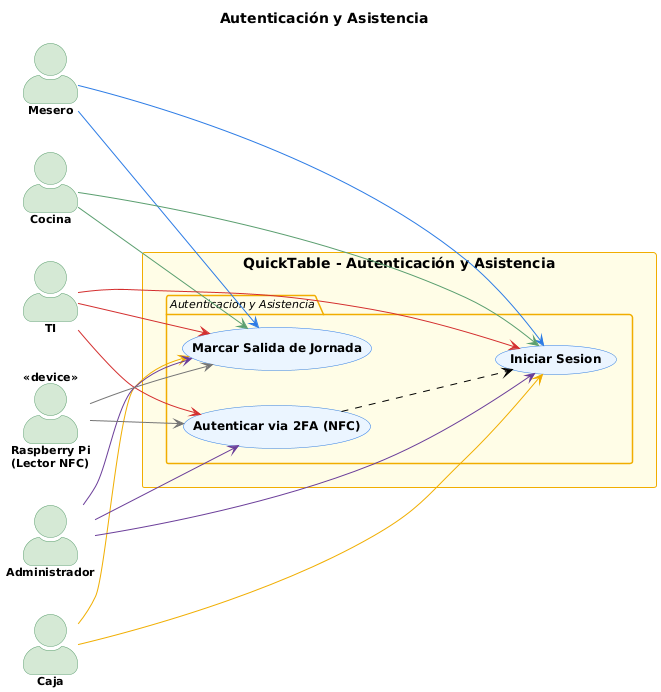
\includegraphics[width=0.8\textwidth]{imagenes/Autenticación y Asistencia.png}
	\caption{Casos de uso de autenticación y registro de asistencia (Realizado con PlantUML)}
	\label{fig:casos_uso_auth}
\end{figure}

La Figura~\ref{fig:casos_uso_auth} muestra los casos de uso relacionados con el inicio y cierre de jornada laboral, así como la autenticación mediante doble factor utilizando tarjetas NFC conectadas a una Raspberry Pi. En esta vista participan todos los roles del sistema, ya que cualquier empleado debe iniciar sesión, autenticarse y marcar la salida de su turno para que la aplicación pueda registrar las jornadas laborales y asociarlas con los pedidos realizados durante el día.

\begin{figure}[H]
	\centering
		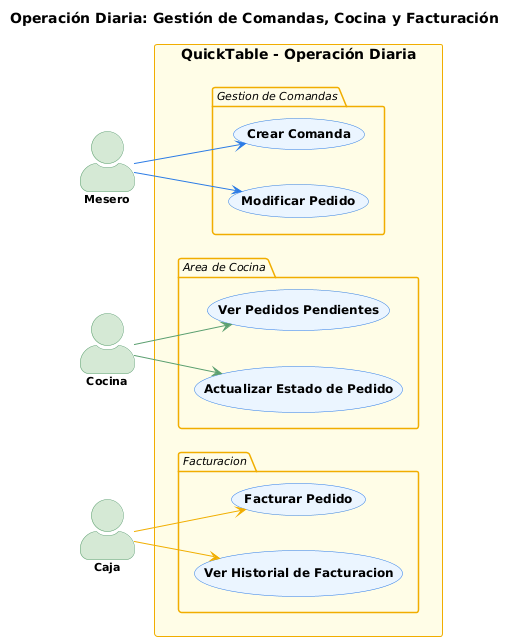
\includegraphics[width=0.75\textwidth]{imagenes/operacion diaria.png}
	\caption{Casos de uso de operación diaria: comandas, cocina y facturación (Realizado con PlantUML)}
	\label{fig:casos_uso_operacion}
\end{figure}

La Figura~\ref{fig:casos_uso_operacion} agrupa los casos de uso asociados a la operación diaria del restaurante: creación y edición de comandas por parte del mesero, gestión del estado de los pedidos en cocina y proceso de facturación en caja. Esta vista se centra en el flujo de una comanda desde que se registra en la mesa, pasa por la preparación en cocina y termina con la emisión de la factura y el cierre de la venta.

\begin{figure}[H]
	\centering
	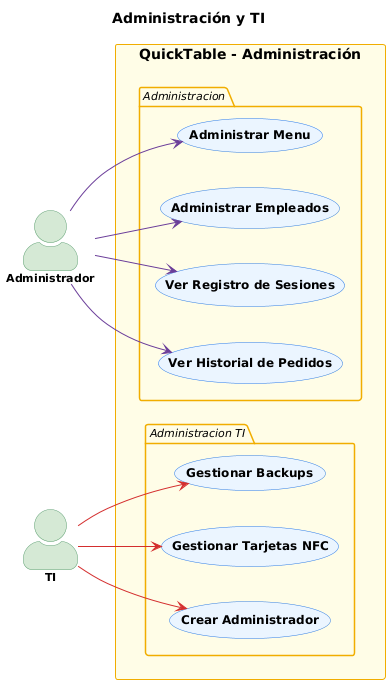
\includegraphics[width=0.6\textwidth]{imagenes/Administracion y ti.png}
	\caption{Casos de uso de administración del sistema y gestión TI (Realizado con PlantUML)}
	\label{fig:casos_uso_admin_ti}
\end{figure}

La Figura~\ref{fig:casos_uso_admin_ti} presenta los casos de uso exclusivos de los roles de Administrador y TI, incluyendo la gestión del menú, empleados, reportes e historial de pedidos, así como la administración de respaldos y de las tarjetas NFC. Estos casos de uso soportan las tareas de configuración, seguridad y mantenimiento del sistema, y están alineados con los módulos de administración y de gestión de tarjetas NFC implementados en la aplicación web.


\subsection{Requerimientos Funcionales (Criterios Given-When-Then)}

Para garantizar una evaluación objetiva durante la fase de pruebas, los requerimientos funcionales más críticos fueron redactados utilizando el formato \textit{Given-When-Then} (Dado-Cuando-Entonces), ampliamente utilizado en escenarios de \textit{Behavior-Driven Development} (BDD) y documentado en publicaciones recientes de IEEE sobre generación automática de casos de prueba a partir de escenarios BDD \cite{Zameni2023,ISO29148:2018}. En este enfoque, cada requerimiento se expresa como una tríada “Dado–Cuando–Entonces” que explicita la precondición, la acción del usuario o del sistema y el resultado esperado.

A continuación, se presentan los requerimientos funcionales principales agrupados por módulo operativo:



\begin{longtable}{|p{2.4cm}|p{4cm}|p{4cm}|p{4.5cm}|}
	\caption{Especificación de Requerimientos Funcionales (Módulos Operativos)} \label{tab:req_funcionales_operativos} \\
	\hline
	\textbf{ID / Módulo} & \textbf{Dado (Given)} & \textbf{Cuando (When)} & \textbf{Entonces (Then)} \\
	\hline
	\endfirsthead
	
	\hline
	\textbf{ID / Módulo} & \textbf{Dado (Given)} & \textbf{Cuando (When)} & \textbf{Entonces (Then)} \\
	\hline
	\endhead
	
	\hline
	\endfoot
	
	\hline
	\endlastfoot
	
	\textbf{RF-01} \newline Acceso al módulo de mesero
	&
	Existe una sesión válida y el usuario autenticado tiene el rol \texttt{Mesero}.
	&
	El usuario intenta ingresar al panel principal o al formulario de nuevo pedido.
	&
	El sistema permite el acceso a las vistas del módulo Mesero; si el rol no corresponde, redirige al \texttt{Index} correspondiente o no existe identificación válida en sesión, redirige al inicio de sesión.
	\\
	\hline
	
	\textbf{RF-02} \newline Creación de pedido
	&
	Un mesero autenticado se encuentra en la vista \texttt{NuevoPedido}, dispone de un número de mesa válido y selecciona al menos un ítem del menú.
	&
	El mesero confirma el pedido enviando la mesa, los ítems, sus cantidades y observaciones.
	&
	El sistema registra el pedido con sus detalles y cálculos financieros, y establece su estado inicial en \texttt{En Preparación}.
	\\
	\hline
	
	\textbf{RF-03} \newline Consulta y filtrado del menú
	&
	El mesero se encuentra creando o editando un pedido y el menú está disponible en la base de datos.
	&
	El usuario busca platos por nombre, filtra por categoría o ajusta cantidades desde la interfaz.
	&
	El sistema muestra los ítems del menú filtrados, permite aumentar o disminuir cantidades y conserva las observaciones digitadas para cada ítem seleccionado.
	\\
	\hline
	
	\textbf{RF-04} \newline Edición de pedido
	&
	Existe un pedido activo asociado al flujo del mesero y sus detalles están disponibles para modificación.
	&
	El mesero ingresa a \texttt{EditarPedido} y confirma cambios en cantidades, ítems u observaciones.
	&
	El sistema actualiza los detalles del pedido existente, recalcula los valores monetarios correspondientes y mantiene el pedido dentro del flujo operativo activo.
	\\
	\hline
	
	\textbf{RF-05} \newline Visualización de pedidos del mesero
	&
	El mesero ha iniciado sesión y existen pedidos activos registrados en el sistema.
	&
	El usuario consulta su panel de pedidos.
	&
	El sistema devuelve los pedidos asociados al mesero autenticado y permite además consultar pedidos de otros meseros mediante los endpoints dispuestos para esa visualización.
	\\
	\hline
	
	\textbf{RF-06} \newline Gestión de pedidos en cocina
	&
	Existen pedidos activos cuyo estado no ha finalizado el flujo de preparación y el usuario autenticado tiene rol \texttt{Cocina}.
	&
	Cocina consulta la vista de pedidos pendientes.
	&
	El sistema lista los pedidos con su número de mesa, identificador y detalles pendientes de preparación, mostrando solo las cantidades aún no preparadas y las observaciones registradas.
	\\
	\hline
	
	\textbf{RF-07} \newline Marcado de pedido listo
	&
	Un pedido activo se encuentra en estado \texttt{En Preparación} o \texttt{Editado} y está disponible en el módulo Cocina.
	&
	El usuario de cocina presiona la opción \texttt{Marcar como Listo}.
	&
	El sistema actualiza el pedido a estado \texttt{Listo}, registra la marca temporal correspondiente y deja el pedido disponible para seguimiento por parte del mesero y caja.
	\\
	\hline
	
	\textbf{RF-08} \newline Aceptación del pedido por el mesero
	&
	Existe un pedido previamente marcado como listo por cocina y visible para el mesero.
	&
	El mesero registra la aceptación del pedido.
	&
	El sistema almacena la fecha y hora de aceptación en el campo \texttt{MeseroAceptadoAt}, permitiendo medir tiempos operativos entre cocina y entrega.
	\\
	\hline
	
	\textbf{RF-09} \newline Consulta de pedidos activos en caja
	&
	El usuario autenticado tiene rol \texttt{Cajero} y existen pedidos activos en el sistema.
	&
	El cajero ingresa al módulo Caja y consulta los pedidos.
	&
	El sistema muestra cada pedido activo con mesa, mesero, estado, subtotal, IVA, total y detalle de productos, permitiendo distinguir visualmente si el pedido está listo o aún en preparación.
	\\
	\hline
	
	\textbf{RF-10} \newline Finalización y cobro del pedido
	&
	Existe un pedido activo seleccionado en caja y el cajero define propina y método de pago.
	&
	El cajero ejecuta la acción \texttt{FinalizarPedido}, indicando además efectivo recibido y cambio cuando aplica.
	&
	El sistema crea un registro en \texttt{HistorialPedido} con sus detalles, subtotal, IVA, total, propina, método de pago, efectivo recibido y cambio; posteriormente elimina el pedido de \texttt{PedidosActivos}.
	\\
	\hline
	
	\textbf{RF-11} \newline Generación de factura
	&
	Un pedido ya fue finalizado correctamente y existe su correspondiente registro en historial.
	&
	El sistema invoca la generación de la factura usando el identificador del pedido histórico.
	&
	El sistema construye la vista \texttt{Factura} con número de pedido, mesa, mesero, fecha, detalle de ítems, subtotal, IVA, propina, total final y método de pago.
	\\
	\hline
	
	\textbf{RF-12} \newline Consulta de historial de pedidos
	&
	Existen pedidos finalizados almacenados en \texttt{HistorialPedido} y el usuario tiene acceso al módulo Caja.
	&
	El cajero consulta el historial y aplica filtros por fecha, número de pedido o ID del mesero.
	&
	El sistema retorna los pedidos paginados del historial con su información general y detalle de productos, conservando los datos del cierre de venta para consulta posterior.
	\\
	\hline
	
\end{longtable}


\subsection{Requerimientos de Seguridad (2FA y Encriptación)}

Dado que uno de los pilares del proyecto es la seguridad y confidencialidad de la información, se establecieron requerimientos funcionales estrictos para el acceso administrativo y la protección de datos:

\begin{longtable}{|p{2.4cm}|p{4cm}|p{4cm}|p{4.5cm}|}
	\caption{Especificación de Requerimientos Funcionales de Seguridad}
	\label{tab:req_funcionales_seguridad} \\
	\hline
	\textbf{ID / Módulo} & \textbf{Dado (Given)} & \textbf{Cuando (When)} & \textbf{Entonces (Then)} \\
	\hline
	\endfirsthead
	
	\hline
	\textbf{ID / Módulo} & \textbf{Dado (Given)} & \textbf{Cuando (When)} & \textbf{Entonces (Then)} \\
	\hline
	\endhead
	
	\hline
	\endfoot
	
	\hline
	\endlastfoot
	
	\textbf{RS-01} \newline Provisión de tarjeta para administrador
	&
	Existe un administrador creado o en proceso de habilitación dentro del módulo de gestión de tarjetas.
	&
	Se solicita registrar o asociar una tarjeta NFC al flujo de acceso administrativo.
	&
	El sistema registra la tarjeta, protege el identificador correspondiente y deja disponible el factor físico necesario para el proceso de validación administrativa.
	\\
	\hline
	
	\textbf{RS-02} \newline Protección de contraseñas
	&
	Se crea un usuario o se actualiza una contraseña en el sistema.
	&
	La contraseña debe almacenarse para autenticaciones futuras.
	&
	El sistema protege la contraseña mediante hashing BCrypt y utiliza el mecanismo de verificación correspondiente cuando el usuario intenta autenticarse.
	\\
	\hline
	
	\textbf{RS-03} \newline Autenticación por credenciales
	&
	Existe un empleado registrado con nombre de usuario y contraseña almacenada.
	&
	El usuario ingresa sus credenciales en el formulario de inicio de sesión.
	&
	El sistema busca el empleado por nombre, valida la contraseña protegida y solo permite continuar el proceso de acceso cuando las credenciales son correctas.
	\\
	\hline
	
	\textbf{RS-04} \newline Doble factor exclusivo para administrador
	&
	Un usuario con rol de \texttt{administrador} ya superó la validación inicial de usuario y contraseña, y existe un proceso de segundo factor asociado a su autenticación.
	&
	El sistema recibe la confirmación del segundo factor mediante el flujo de \texttt{Confirmar2FA} y consulta su estado con \texttt{Check2FA}.
	&
	El sistema concede el acceso administrativo únicamente cuando el segundo factor ha sido confirmado correctamente; este control reforzado aplica al administrador.
	\\
	\hline
	
	\textbf{RS-05} \newline Validación de sesión para hardware
	&
	Existe un código de sesión generado para un flujo de validación con dispositivo o tarjeta NFC.
	&
	El cliente o dispositivo envía el código de sesión a los mecanismos de validación definidos para administrador o empleado.
	&
	El sistema verifica el formato y la vigencia del código, y autoriza la operación solo si la sesión correspondiente es válida.
	\\
	\hline
	
	\textbf{RS-06} \newline Control de acceso por rol
	&
	Existe una sesión iniciada o un usuario intenta acceder a un módulo protegido.
	&
	El usuario intenta ingresar a una vista o acción restringida a un rol específico.
	&
	El sistema valida el rol almacenado en sesión y permite el acceso únicamente al módulo autorizado; en caso contrario, redirige al inicio de sesión o rechaza la solicitud.
	\\
	\hline
	
	\textbf{RS-07} \newline Gestión segura de sesión
	&
	Un usuario autenticado inicia o mantiene una sesión activa en la aplicación.
	&
	El sistema crea, conserva o finaliza la sesión del usuario.
	&
	El sistema registra conexión y desconexión, configura la sesión mediante cookie \texttt{HttpOnly}, aplica expiración por inactividad y limpia procesos pendientes al cerrar sesión.
	\\
	\hline
	
\end{longtable}


\subsection{Requerimientos No Funcionales}

Además de las funcionalidades, el diseño del sistema debió contemplar restricciones técnicas que garantizaran su viabilidad operativa, seguridad, mantenibilidad y bajo costo de implementación, considerando las capacidades tecnológicas habituales de los restaurantes PYME.

\begin{itemize}
	\item \textbf{Multiplataforma:} La interfaz de usuario debe ser accesible y responsiva desde dispositivos móviles (smartphones y tablets) y computadores de escritorio mediante navegadores web modernos, evitando la necesidad de instalar aplicaciones nativas.
	
	\item \textbf{Despliegue Local (Intranet):} El sistema debe operar sobre una red local del establecimiento, sin depender de una conexión permanente a internet para ejecutar sus funciones principales.
	
	\item \textbf{Tiempos de Respuesta:} Las operaciones de consulta, registro y actualización de comandas deben ejecutarse con tiempos de respuesta suficientemente bajos para no afectar el flujo operativo del restaurante, idealmente en menos de 2 segundos por transacción.
	
	\item \textbf{Optimización de Recursos:} El backend y la base de datos deben poder ejecutarse sobre hardware de gama de entrada, con el fin de mantener bajos los costos de adopción para pequeñas y medianas empresas.
	
	\item \textbf{Seguridad de Sesión:} El sistema debe administrar sesiones de usuario con mecanismos que reduzcan accesos no autorizados, incluyendo expiración por inactividad y uso de cookies seguras de sesión.
	
	\item \textbf{Protección de Datos Sensibles:} La información sensible, como credenciales y datos asociados a mecanismos de autenticación, debe almacenarse utilizando técnicas de protección criptográfica apropiadas.
	
	\item \textbf{Respaldo y Recuperación:} El sistema debe permitir la generación y restauración de copias de seguridad para proteger la información operativa frente a fallos del sistema o pérdida de datos.
	
	\item \textbf{Mantenibilidad:} La solución debe conservar una estructura modular que facilite la corrección de errores, la evolución del sistema y la incorporación de nuevas funcionalidades sin afectar los componentes ya implementados.
	
	\item \textbf{Trazabilidad Operativa:} El sistema debe registrar eventos relevantes de acceso y cierre de sesión para facilitar el control administrativo y el seguimiento de la operación diaria.
\end{itemize}




%\subsection{Casos de Uso}
% Aquí puedes incluir un diagrama de casos de uso general y explicar los roles: Administrador, Mesero, Cocina, Caja y TI.
% Ejemplo de figura para el diagrama de casos de uso:
% \begin{figure}[H]
	%     \centering
	%     
\includegraphics[width=0.8\textwidth]{casos_uso.png}
	%     \caption{Diagrama general de casos de uso del sistema}
	%     \label{fig:casos_uso}
	% \end{figure}

\subsection{Arquitectura General del Sistema}
Para el desarrollo de la aplicación se implementó una arquitectura cliente-servidor basada en el modelo de tres capas: Presentación, Lógica de Negocio y Datos. Esta estructura garantiza la separación de responsabilidades, facilitando la escalabilidad, el mantenimiento del código y la seguridad del sistema. El patrón arquitectónico principal utilizado fue el Modelo-Vista-Controlador (MVC), adaptado mediante la tecnología Razor Pages de .NET 8, la cual encapsula el modelo y el controlador en una clase unificada (\texttt{PageModel}) vinculada directamente a su respectiva vista, optimizando el flujo de trabajo en aplicaciones orientadas a páginas.

La arquitectura general se compone de los siguientes elementos:

\begin{itemize}
	\item \textbf{Capa de Presentación (Frontend):} Desarrollada utilizando HTML5, CSS3, JavaScript y el framework Bootstrap. La interfaz de usuario toma como base estructural la plantilla AdminLTE, la cual fue extendida y fuertemente personalizada para adaptar la apariencia a las necesidades visuales y operativas del sistema en dispositivos móviles y de escritorio.
	\item \textbf{Capa de Aplicación (Backend):} Construida con el framework .NET 8 en el lenguaje C\#. Es responsable de procesar las peticiones HTTP, ejecutar las reglas de negocio y gestionar la comunicación con el módulo de hardware RFID mediante Endpoints de API tipo REST.
	\item \textbf{Capa de Datos:} Implementada sobre el motor de base de datos relacional Microsoft SQL Server, utilizando el ORM Entity Framework 6 (EF6) para garantizar una comunicación segura y transaccional.
	\item \textbf{Módulo de Seguridad (Hardware):} Compuesto por una Raspberry Pi interactuando con un lector NFC RFID-RC522, el cual actúa como un cliente independiente para la validación física del administrador en el esquema de doble factor de autenticación (2FA).
\end{itemize}

% diagrama de bloques
\begin{figure}[H]
	\centering
	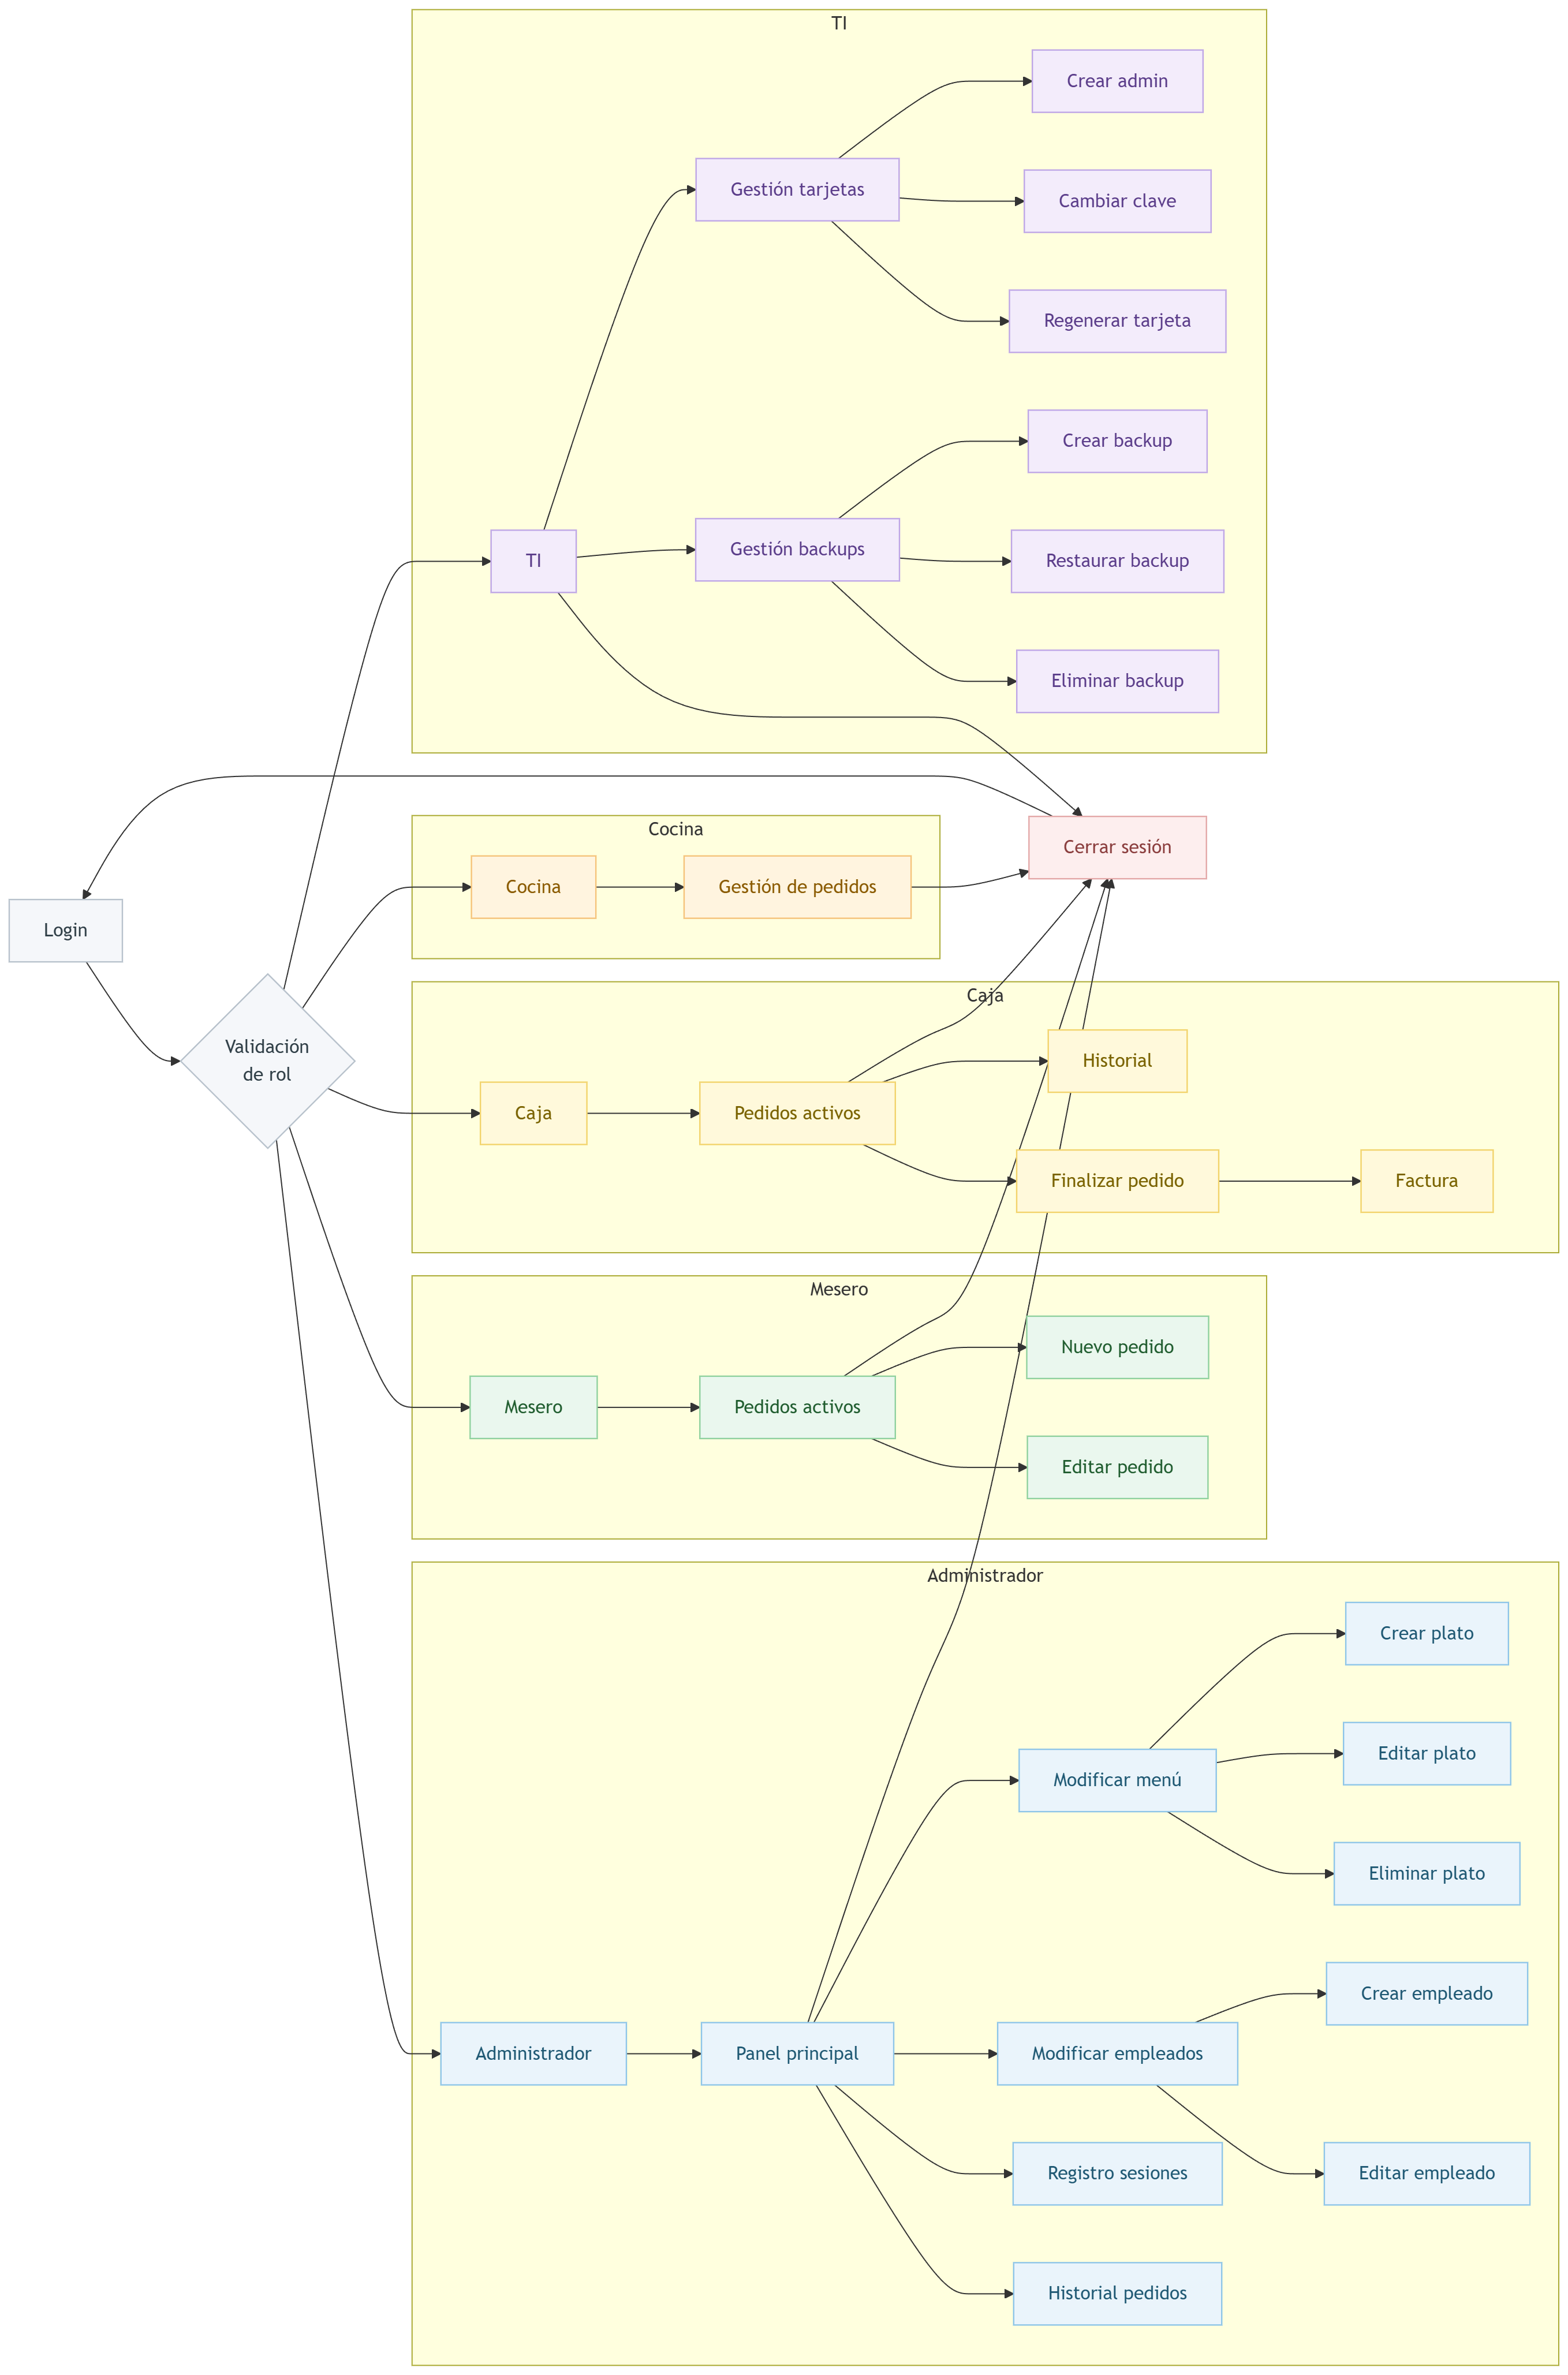
\includegraphics[width=0.9\textwidth]{imagenes/arquitectura_bloques.png}
	\caption{Diagrama de bloques de la arquitectura del sistema}
	\label{fig:arquitectura_bloques}
\end{figure}


\section{Diseño e Implementación de la Base de Datos}

El diseño de la base de datos se estructuró para soportar las operaciones críticas del restaurante de manera transaccional, garantizando la integridad referencial y minimizando la redundancia de datos. Se optó por el motor Microsoft SQL Server debido a su robustez, soporte nativo de encriptación y excelente integración con el ecosistema de desarrollo de Microsoft.

\subsection{Modelo Entidad-Relación}

El esquema de la base de datos consta de tablas interrelacionadas que representan las entidades fundamentales del negocio y los mecanismos de seguridad. Entre las entidades principales se encuentran:

\begin{itemize}
	\item \textbf{Empleados:} Almacena las credenciales protegidas (mediante hashing BCrypt) de los usuarios, sus datos personales, el UID asociado (si aplica) y el rol asignado dentro del sistema (Admin, Mesero, Cocina, Cajero).
	\item \textbf{MenuItems (Menú):} Contiene el catálogo de productos disponibles, sus descripciones, categorías y precios, permitiendo la construcción dinámica de los pedidos.
	\item \textbf{PedidosActivos e ItemDetalle:} Tablas transaccionales encargadas de almacenar el encabezado de la comanda en curso (fecha, mesero, mesa, totales y estado de preparación) y los ítems individuales con sus cantidades y observaciones, respectivamente.
	\item \textbf{HistorialPedidos e HistorialDetalle:} Entidades destinadas a la persistencia de las comandas ya facturadas y finalizadas, garantizando la inmutabilidad de los datos históricos de ventas y facturación.
	\item \textbf{TarjetasRC:} Tabla dedicada a la seguridad por hardware, que almacena el UID físico de las tarjetas NFC y gestiona la asignación activa a los usuarios administradores.
	\item \textbf{RegistroSesiones y Codigos2FA:} Entidades de auditoría y control de acceso. La primera registra las horas de conexión y desconexión de los empleados para el control de asistencia, mientras que la segunda gestiona de forma temporal los tokens para la autenticación de doble factor.
\end{itemize}

 \begin{figure}[H] 
	 	\centering
	 	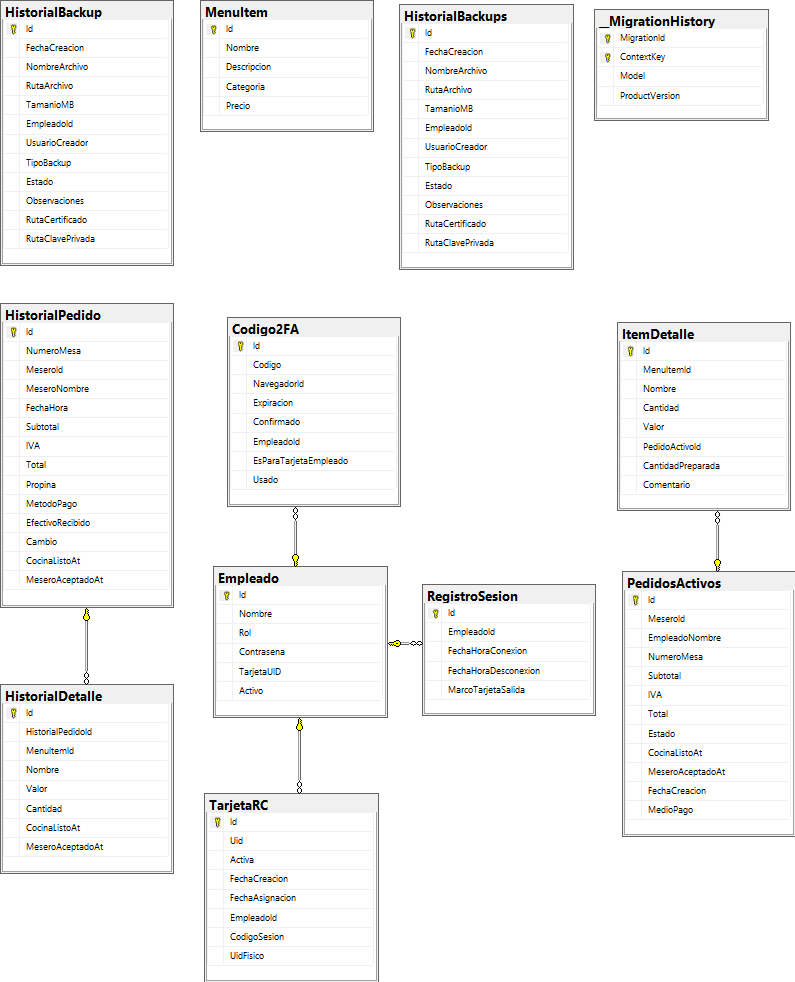
\includegraphics[width=0.95\textwidth]{imagenes/diagrama_mer.png}
	 	\caption{Modelo Entidad-Relación de la base de datos (Creado en SMSS 20)}
	 	\label{fig:diagrama_mer}
	 \end{figure}

Como se observa en la Figura \ref{fig:diagrama_mer}, el modelo de datos fue diseñado siguiendo un enfoque relacional normalizado que separa claramente la operación en tiempo real de la persistencia histórica. La entidad central del sistema es \textbf{Empleado}, la cual establece una relación de 'uno a muchos' tanto con los \textbf{PedidosActivos} como con el \textbf{RegistroSesion}, permitiendo la trazabilidad de qué usuario (Mesero) crea cada comanda y en qué horarios labora el personal. Asimismo, mantiene una relación opcional de 'uno a uno' con la tabla \textbf{TarjetaRC}, utilizada exclusivamente para vincular credenciales físicas NFC a los perfiles con rol de Administrador.

El flujo transaccional del restaurante se maneja a través de dos estructuras gemelas: una para la operación en curso y otra para el archivo histórico. Un \textbf{PedidoActivo} actúa como entidad cabecera que se relaciona de 'uno a muchos' con \textbf{ItemDetalle}, donde cada detalle hace referencia mediante llave foránea al producto específico en la tabla \textbf{MenuItem}. Una vez que el Cajero procesa el pago y finaliza la orden, la integridad de los datos se garantiza migrando la información hacia las entidades \textbf{HistorialPedido} e \textbf{HistorialDetalle}. Esta separación arquitectónica evita la sobrecarga de la tabla de pedidos activos, garantizando tiempos de respuesta rápidos (menores a 2 segundos) para el personal de Meseros y Cocina, mientras se conservan los datos inmutables de facturación para consultas administrativas.

\subsection{Implementación con Entity Framework 6}
La arquitectura de persistencia de datos del sistema fue implementada utilizando Entity Framework 6 (EF6) bajo el ecosistema de .NET 8. Se optó por EF6 debido a su alta madurez y estabilidad a nivel empresarial. Al contar con una extensa documentación y un motor de persistencia rigurosamente probado contra fallos transaccionales, se reduce la curva de aprendizaje para futuros mantenimientos, alineándose con el objetivo de ofrecer una solución escalable y de bajo costo para las PYMES.

Para gestionar la interacción con la base de datos, el sistema define un contexto principal denominado \texttt{SistemaQuickTableContext}, el cual hereda de la clase base \texttt{DbContext}. La persistencia se estructura bajo los siguientes principios:

\begin{itemize}
	\item \textbf{Mapeo Objeto-Relacional Consolidado:} Las tablas de SQL Server se representan directamente mediante entidades (clases) ubicadas en el directorio \texttt{Dominio} (ej. \texttt{PedidoActivo}, \texttt{ItemDetalle}). El contexto administra el estado de estas entidades a través de colecciones \texttt{DbSet<T>}, garantizando que las modificaciones en la lógica de negocio se traduzcan de manera íntegra a la base de datos.
	\item \textbf{Gestión Segura de Conexiones:} La cadena de conexión al motor SQL Server se inyecta dinámicamente desde el archivo de configuración \texttt{appsettings.json}. Esta separación aísla las credenciales de acceso del código fuente principal, cumpliendo con las buenas prácticas de seguridad informática.
	\item \textbf{Abstracción de Consultas con LINQ:} Las operaciones CRUD ejecutadas por los diferentes módulos no emplean sentencias SQL estáticas. En su lugar, se utiliza \textit{Language Integrated Query} (LINQ), lo cual mitiga por diseño las vulnerabilidades de inyección SQL y optimiza la legibilidad del código al expresar reglas de negocio en lenguaje nativo C\#.
\end{itemize}


\section{Implementación de la Solución Web}

El núcleo central del sistema fue desarrollado como una aplicación web robusta, diseñada para centralizar la comunicación entre las áreas del restaurante y eliminar las ineficiencias del papel. El desarrollo se fundamentó en el ecosistema de Microsoft, utilizando .NET 8 y el patrón arquitectónico MVC (Modelo-Vista-Controlador) adaptado mediante el enfoque de \textit{Razor Pages}.

\subsection{Interfaz de Usuario (Frontend y Personalización visual)}

Como se estableció en el diseño arquitectónico, la capa de presentación toma como base estructural el framework \textbf{AdminLTE} (soportado por Bootstrap). Sin embargo, su implementación no se limitó al uso genérico de la plantilla; esta fue sometida a una \textbf{reestructuración y personalización profunda mediante hojas de estilo propias (CSS)}. El objetivo de esta sobreescritura de estilos fue transformar un panel de control administrativo estándar en una interfaz operativa ágil, adaptada específicamente a las condiciones físicas del sector gastronómico.

Esta implementación personalizada aportó las siguientes características técnicas al proyecto:

\begin{itemize}
	\item \textbf{Diseño Responsivo y Optimización Táctil:} Si bien la estructura de grillas de Bootstrap garantiza la adaptabilidad a diferentes resoluciones, el CSS personalizado se enfocó en ampliar las áreas de interacción (botones, selectores de cantidad y tarjetas de menú). Esto es vital para facilitar la precisión táctil en los \textit{smartphones} de los meseros y evitar toques accidentales durante operaciones rápidas.
	\item \textbf{Minimalismo y Contraste Visual:} Se sobrescribieron los estilos predeterminados de AdminLTE para ocultar elementos modulares innecesarios (como menús laterales complejos) en las vistas operativas. Asimismo, se implementó una paleta de colores de alto contraste que permite a los cocineros y cajeros identificar visualmente y a distancia el estado de un pedido (por ejemplo, alertas visuales para comandas en espera prolongada o listas para entrega).
	\item \textbf{Interactividad Asíncrona:} Para complementar el diseño visual, se integró JavaScript (junto con librerías como jQuery y DataTables) en las vistas de Razor Pages. Esto permitió habilitar acciones dinámicas sin necesidad de recargar la página completa, optimizando tiempos muertos al momento de filtrar el menú o actualizar el estado de preparación de un plato.
\end{itemize}


\subsection{Lógica de Negocio y Módulos .NET 8 (Razor Pages)}
El backend de la aplicación gestiona la lógica de negocio a través del enfoque de Razor Pages, el cual agrupa los controladores y las vistas en un diseño orientado a páginas (\textit{Page-Focused}), resultando en un código más organizado y fácil de mantener que el MVC tradicional para este tipo de aplicaciones. 

El sistema fue segmentado en cinco módulos principales, protegidos por un sistema de autorización basado en reclamaciones (\textit{Claims}) que restringe el acceso según el rol del empleado autenticado:

\begin{itemize}
	\item \textbf{Módulo de Meseros:} Implementa el modelo \texttt{PageModel} para recibir peticiones HTTP POST con objetos JSON que contienen los arreglos de productos. El controlador procesa la lógica matemática de impuestos y subtotales en el servidor y ejecuta la persistencia inicial del registro en la tabla \texttt{PedidosActivos}.
	\item \textbf{Módulo de Cocina:} Funciona mediante consultas asíncronas periódicas (AJAX) que interrogan a la base de datos para extraer dinámicamente los registros con estado pendiente. A través de Endpoints específicos, permite la actualización de estados y marcas temporales sin necesidad de recargar el DOM completo.
	\item \textbf{Módulo de Caja:} Su controlador gestiona el ciclo de vida final del objeto pedido. Tras la confirmación del pago mediante peticiones asíncronas, el sistema ejecuta la lógica transaccional de migración de datos, trasladando la información desde las tablas operativas (\texttt{PedidosActivos}) hacia las entidades inmutables del esquema (\texttt{HistorialPedidos}).
	\item \textbf{Módulos de Administración y TI:} Exponen las interfaces de configuración del CRUD de inventarios y empleados, y gestionan los algoritmos criptográficos (hashing de credenciales). Además, orquestan la comunicación externa exponiendo los Endpoints REST de la API que interactúan con la Raspberry Pi para la verificación de tarjetas NFC.
\end{itemize}


% Descomentar y ajustar cuando tengas pantallazos del sistema
% \begin{figure}[H]
	%     \centering
	%     \includegraphics[width=0.85\textwidth]{imagenes/interfaz_mesero.png}
	%     \caption{Interfaz de usuario del módulo de mesero (diseño responsivo)}
	%     \label{fig:interfaz_mesero}
	% \end{figure}

\subsection{Análisis Visual de la Interfaz Implementada}

Para validar el cumplimiento de los requerimientos de usabilidad y la correcta aplicación de los estilos CSS personalizados sobre AdminLTE, se desarrollaron esquemas visuales comentados a partir de las interfaces finales del sistema. Estos diagramas evidencian las decisiones de diseño enfocadas en la operación rápida y la visualización en diferentes dispositivos (Figura \ref{fig:interfaz_mesero_anotada} y Figura \ref{fig:interfaz_cocina_anotada}).

En la vista destinada al personal de servicio (Meseros), se priorizó el diseño \textit{Mobile-First}, maximizando las áreas táctiles para la selección de platos y el ajuste de cantidades. Se implementaron tarjetas (\textit{cards}) individuales para cada ítem del menú, facilitando su lectura en pantallas reducidas.

\begin{figure}[H]
	\centering
	% Sugerencia: Una imagen de un celular mostrando la toma de pedidos con flechas apuntando a los botones grandes.
	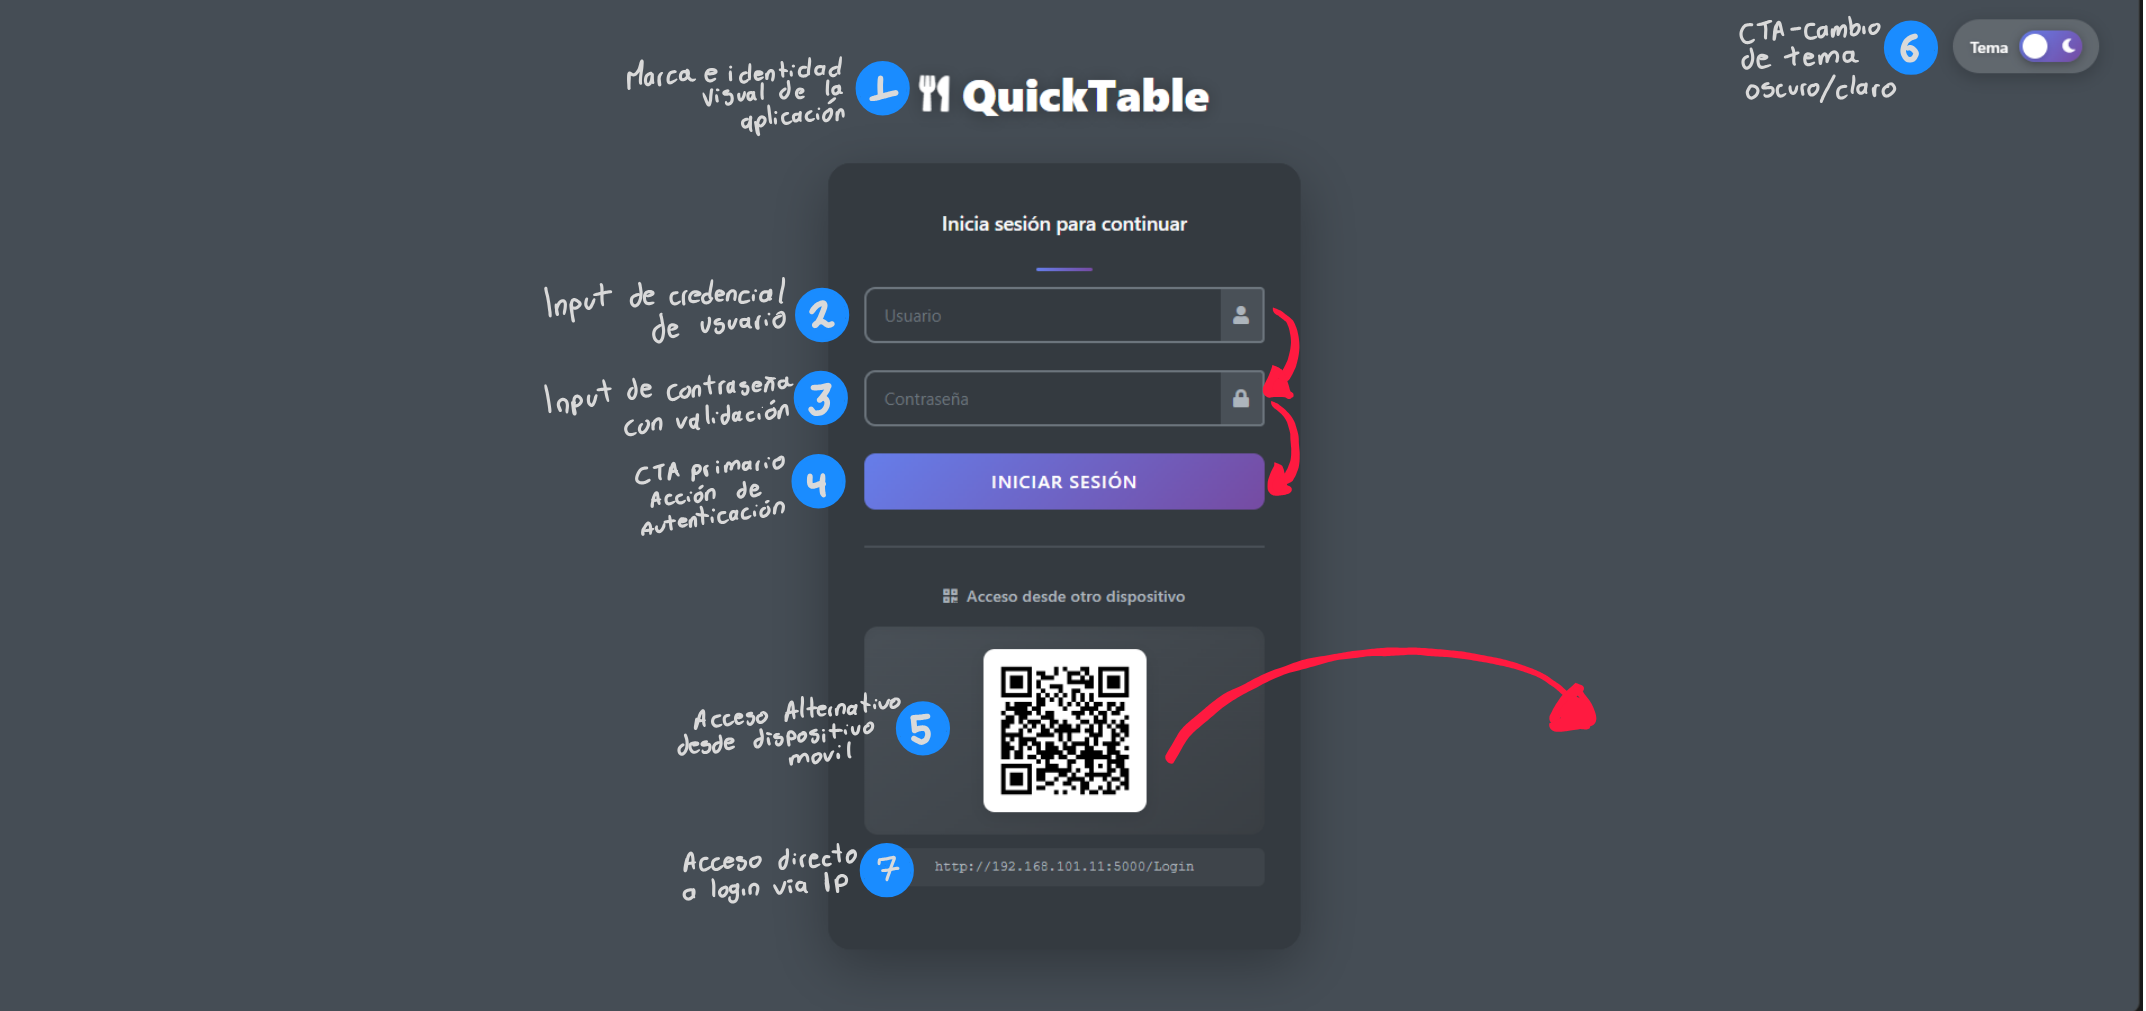
\includegraphics[width=0.85\textwidth]{imagenes/mockup_mesero.png} 
	\caption{CAMBIAR.}
	\label{fig:interfaz_mesero_anotada}
\end{figure}

Por otro lado, la vista del módulo de Cocina fue diseñada para su visualización en pantallas de formato horizontal (monitores o tablets en formato apaisado). Como se observa en la distribución de los componentes, la interfaz minimiza la interacción física requerida por parte del cocinero, mostrando la información estructurada por comandas entrantes y utilizando un código de colores de alto contraste para identificar el estado de preparación de los alimentos.

\begin{figure}[H]
	\centering
	% Sugerencia: Una imagen de la pantalla de cocina (monitor) con notas sobre los colores de estado y el botón "Marcar Listo".
	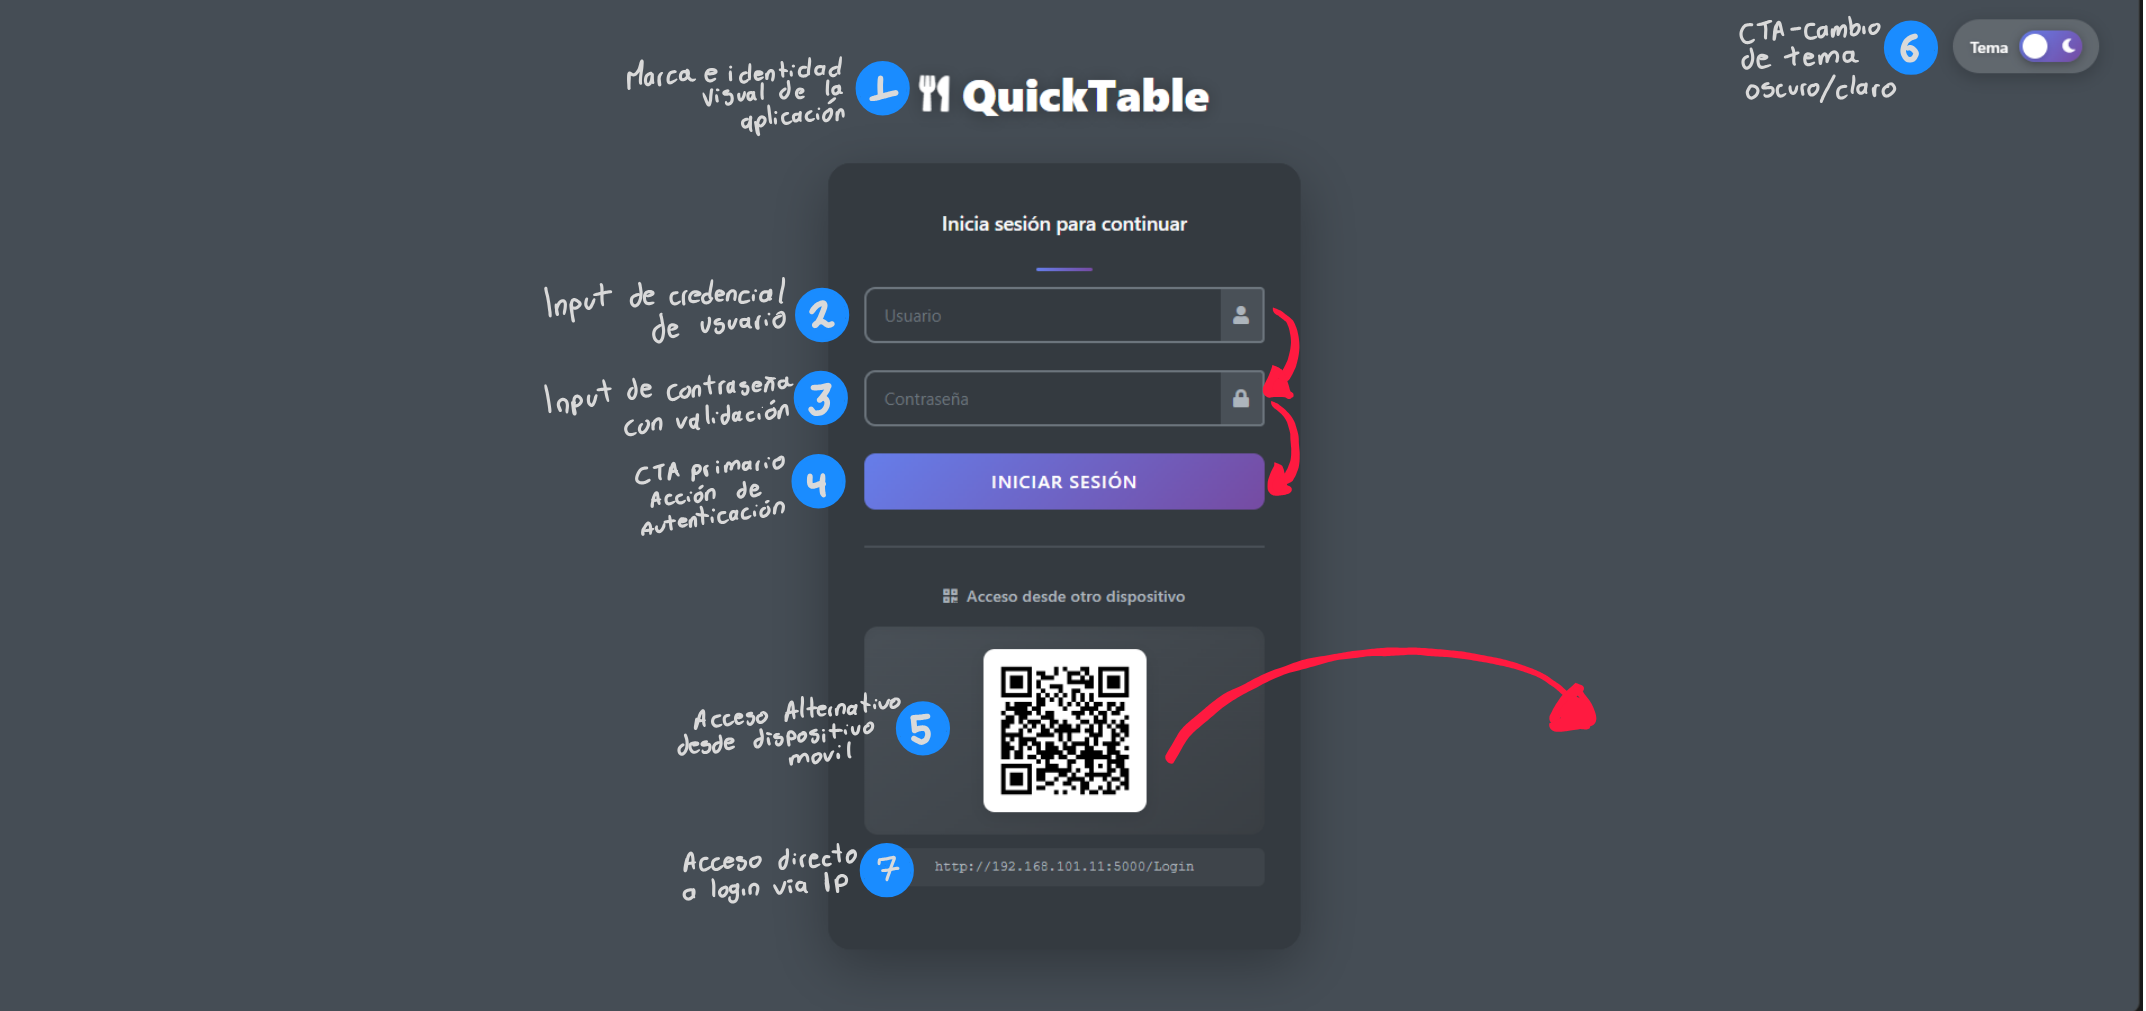
\includegraphics[width=0.9\textwidth]{imagenes/mockup_mesero.png} 
	\caption{CAMBIAR}
	\label{fig:interfaz_cocina_anotada}
\end{figure}





\section{Implementación del Módulo de Seguridad por Hardware (2FA Local)}

En el contexto del desarrollo de aplicaciones web contemporáneas, la implementación de mecanismos de Autenticación de Doble Factor (2FA) se ha estandarizado mediante el uso de servicios basados en la nube, tales como el envío de tokens por SMS, correos electrónicos o aplicaciones generadoras de códigos (ej. Microsoft Authenticator). Sin embargo, en el marco de este proyecto, dichos métodos presentan un obstáculo técnico restrictivo: \textbf{su dependencia de una conexión activa a Internet}.

Dado que uno de los requerimientos no funcionales prioritarios del sistema es garantizar su funcionamiento ininterrumpido sobre una red local (Intranet) con el fin de reducir los costos operativos mensuales para el establecimiento, se descartó la integración de sistemas 2FA en la nube. En su lugar, se diseñó e implementó un módulo de seguridad por hardware basado en tecnología NFC (\textit{Near Field Communication}). Este enfoque añade una capa de seguridad basada en un factor físico de posesión ('algo que el usuario tiene'), garantizando la presencia in situ del administrador al momento de autorizar accesos críticos, operando de manera 100\% \textit{offline} e integrándose de forma nativa con el servidor .NET 8.

\subsection{Arquitectura y Configuración del Hardware}

El dispositivo de validación física actúa como un cliente independiente dentro de la red local del restaurante. Su arquitectura de hardware se compone de dos elementos principales:

\begin{itemize}
	\item \textbf{Unidad de Procesamiento:} Se utilizó una placa \textit{Raspberry Pi 3 Model B v1.2}, la cual ofrece conectividad de red local (Wi-Fi/Ethernet) y los pines de propósito general (GPIO) necesarios para la interacción con periféricos externos.
	\item \textbf{Lector RFID/NFC:} Se integró el módulo \textit{RFID-RC522}, que opera a una frecuencia de 13.56 MHz. Este sensor fue seleccionado por su bajo costo, bajo consumo energético y alta fiabilidad en entornos comerciales.
\end{itemize}

La comunicación entre la Raspberry Pi y el lector RC522 se estableció mediante el protocolo de comunicación síncrona \textbf{SPI} (\textit{Serial Peripheral Interface}). Se configuraron los pines físicos correspondientes (MOSI, MISO, SCK, SDA y RST) para garantizar una transmisión de datos rápida y libre de interferencias al momento de leer el identificador único (UID) de las tarjetas asignadas a los administradores.

\subsection{Desarrollo del Cliente Python e Interfaz Gráfica (Tkinter)}
Para gobernar el comportamiento del hardware de validación física, se desarrolló un script en Python 3 que se ejecuta localmente en la Raspberry Pi. Este lenguaje fue seleccionado por su alta compatibilidad con el sistema operativo (Raspberry Pi OS) y la madurez de sus librerías para la manipulación de los puertos GPIO.

Para optimizar la interacción del usuario sin requerir periféricos externos como teclados o ratones, el dispositivo fue dotado de una Interfaz Gráfica de Usuario (GUI) orientada a pantallas táctiles, desarrollada con la librería estándar \texttt{Tkinter}. El diseño presenta un teclado numérico renderizado en pantalla (\textit{numpad}), permitiendo al administrador digitar un código de sesión dinámico temporal que vincula la lectura física de la tarjeta NFC con el intento de inicio de sesión en el navegador web.

El funcionamiento interno del programa se apoya en la integración concurrente de tres librerías fundamentales:
\begin{enumerate}
	\item \textbf{Tkinter (GUI):} Encargada de la construcción visual y de capturar las pulsaciones del usuario en la pantalla táctil mediante su bucle principal de eventos (\textit{mainloop}).
	\item \textbf{mfrc522 (Hardware):} Librería especializada que inicializa la comunicación por el bus SPI, activa el campo electromagnético del sensor RC522 y extrae el identificador único (UID) crudo de las tarjetas NFC.
	\item \textbf{Requests (Red):} Biblioteca HTTP de alto nivel utilizada para empaquetar el UID leído y el código de sesión en formato JSON, formulando una petición HTTP \texttt{POST} asíncrona hacia el Endpoint REST del servidor .NET 8 (ej. \texttt{/api/auth/validate-nfc}).
\end{enumerate}

Uno de los principales retos técnicos en este script fue evitar el bloqueo (\textit{freezing}) de la interfaz gráfica durante el proceso de lectura. Dado que la función de lectura de la librería \texttt{mfrc522} es bloqueante (espera indefinidamente hasta detectar una tarjeta), ejecutarla en el hilo principal detendría la pantalla. Para solucionar esto, se implementó un modelo de programación concurrente mediante \textit{Threading}. Al confirmar el código de sesión, la GUI delega la lectura NFC y la transmisión HTTP a un hilo secundario (\textit{Worker Thread}). Así, la interfaz sigue respondiendo y mostrando retroalimentación visual ("Esperando tarjeta...") hasta que el servidor retorna un código de estado HTTP (200 OK o 401 Unauthorized), concluyendo el ciclo de comunicación.


\subsection{Sincronización y Criptografía con el Backend (.NET 8)}

El éxito operativo de este módulo radica en su perfecta sincronización con la capa de aplicación web, diseñada bajo estrictos controles de seguridad perimetral. 

Cuando el UID de la tarjeta es recibido por el servidor a través del \textit{Endpoint} de la API, el sistema .NET 8 no lo procesa ni lo almacena en texto plano. El backend recupera el UID encriptado de la base de datos (protegido previamente mediante algoritmos de cifrado simétrico) asociado al perfil del administrador en cuestión. Si la validación criptográfica es exitosa y el código de sesión coincide con una solicitud web activa y no expirada, el servidor actualiza el estado de los reclamos (\textit{Claims}) de autenticación del usuario a 'Autorizado'.

De manera simultánea, la vista del navegador en la estación de trabajo realiza consultas asíncronas periódicas mediante JavaScript (método de \textit{polling}) para verificar su estado. Al detectar la autorización emitida por la Raspberry Pi, el sistema redirige automáticamente al administrador a su panel de control privado, completando el ciclo de validación sin necesidad de exponer credenciales o tokens a redes externas.


\subsection{Diagrama de Secuencia UML: Flujo de Autenticación 2FA}

Para ilustrar de manera formal la interacción entre los diferentes componentes de la arquitectura durante el proceso de autenticación más crítico del sistema (el doble factor mediante hardware), se desarrolló un Diagrama de Secuencia basado en el estándar UML (Lenguaje Unificado de Modelado). 

Como se detalló en los apartados anteriores, la validación no recae en un solo componente, sino que es el resultado de un flujo de comunicación asíncrona y orquestada entre el navegador del usuario (Frontend web), el servidor central (.NET 8), la base de datos (SQL Server) y el dispositivo físico (Raspberry Pi). 

En la Figura \ref{fig:uml_secuencia_2fa} se expone la cronología de los mensajes y peticiones que se ejecutan desde el momento en que el administrador ingresa sus credenciales primarias, la posterior generación del código de sesión dinámico, el proceso de espera mediante la técnica de \textit{polling} en JavaScript, la interrupción del hilo secundario en Python tras la lectura NFC, y finalmente, la resolución criptográfica de los datos (comparación de \textit{Hashes}) que autoriza la concesión del acceso.

\begin{figure}[H]
	\centering
	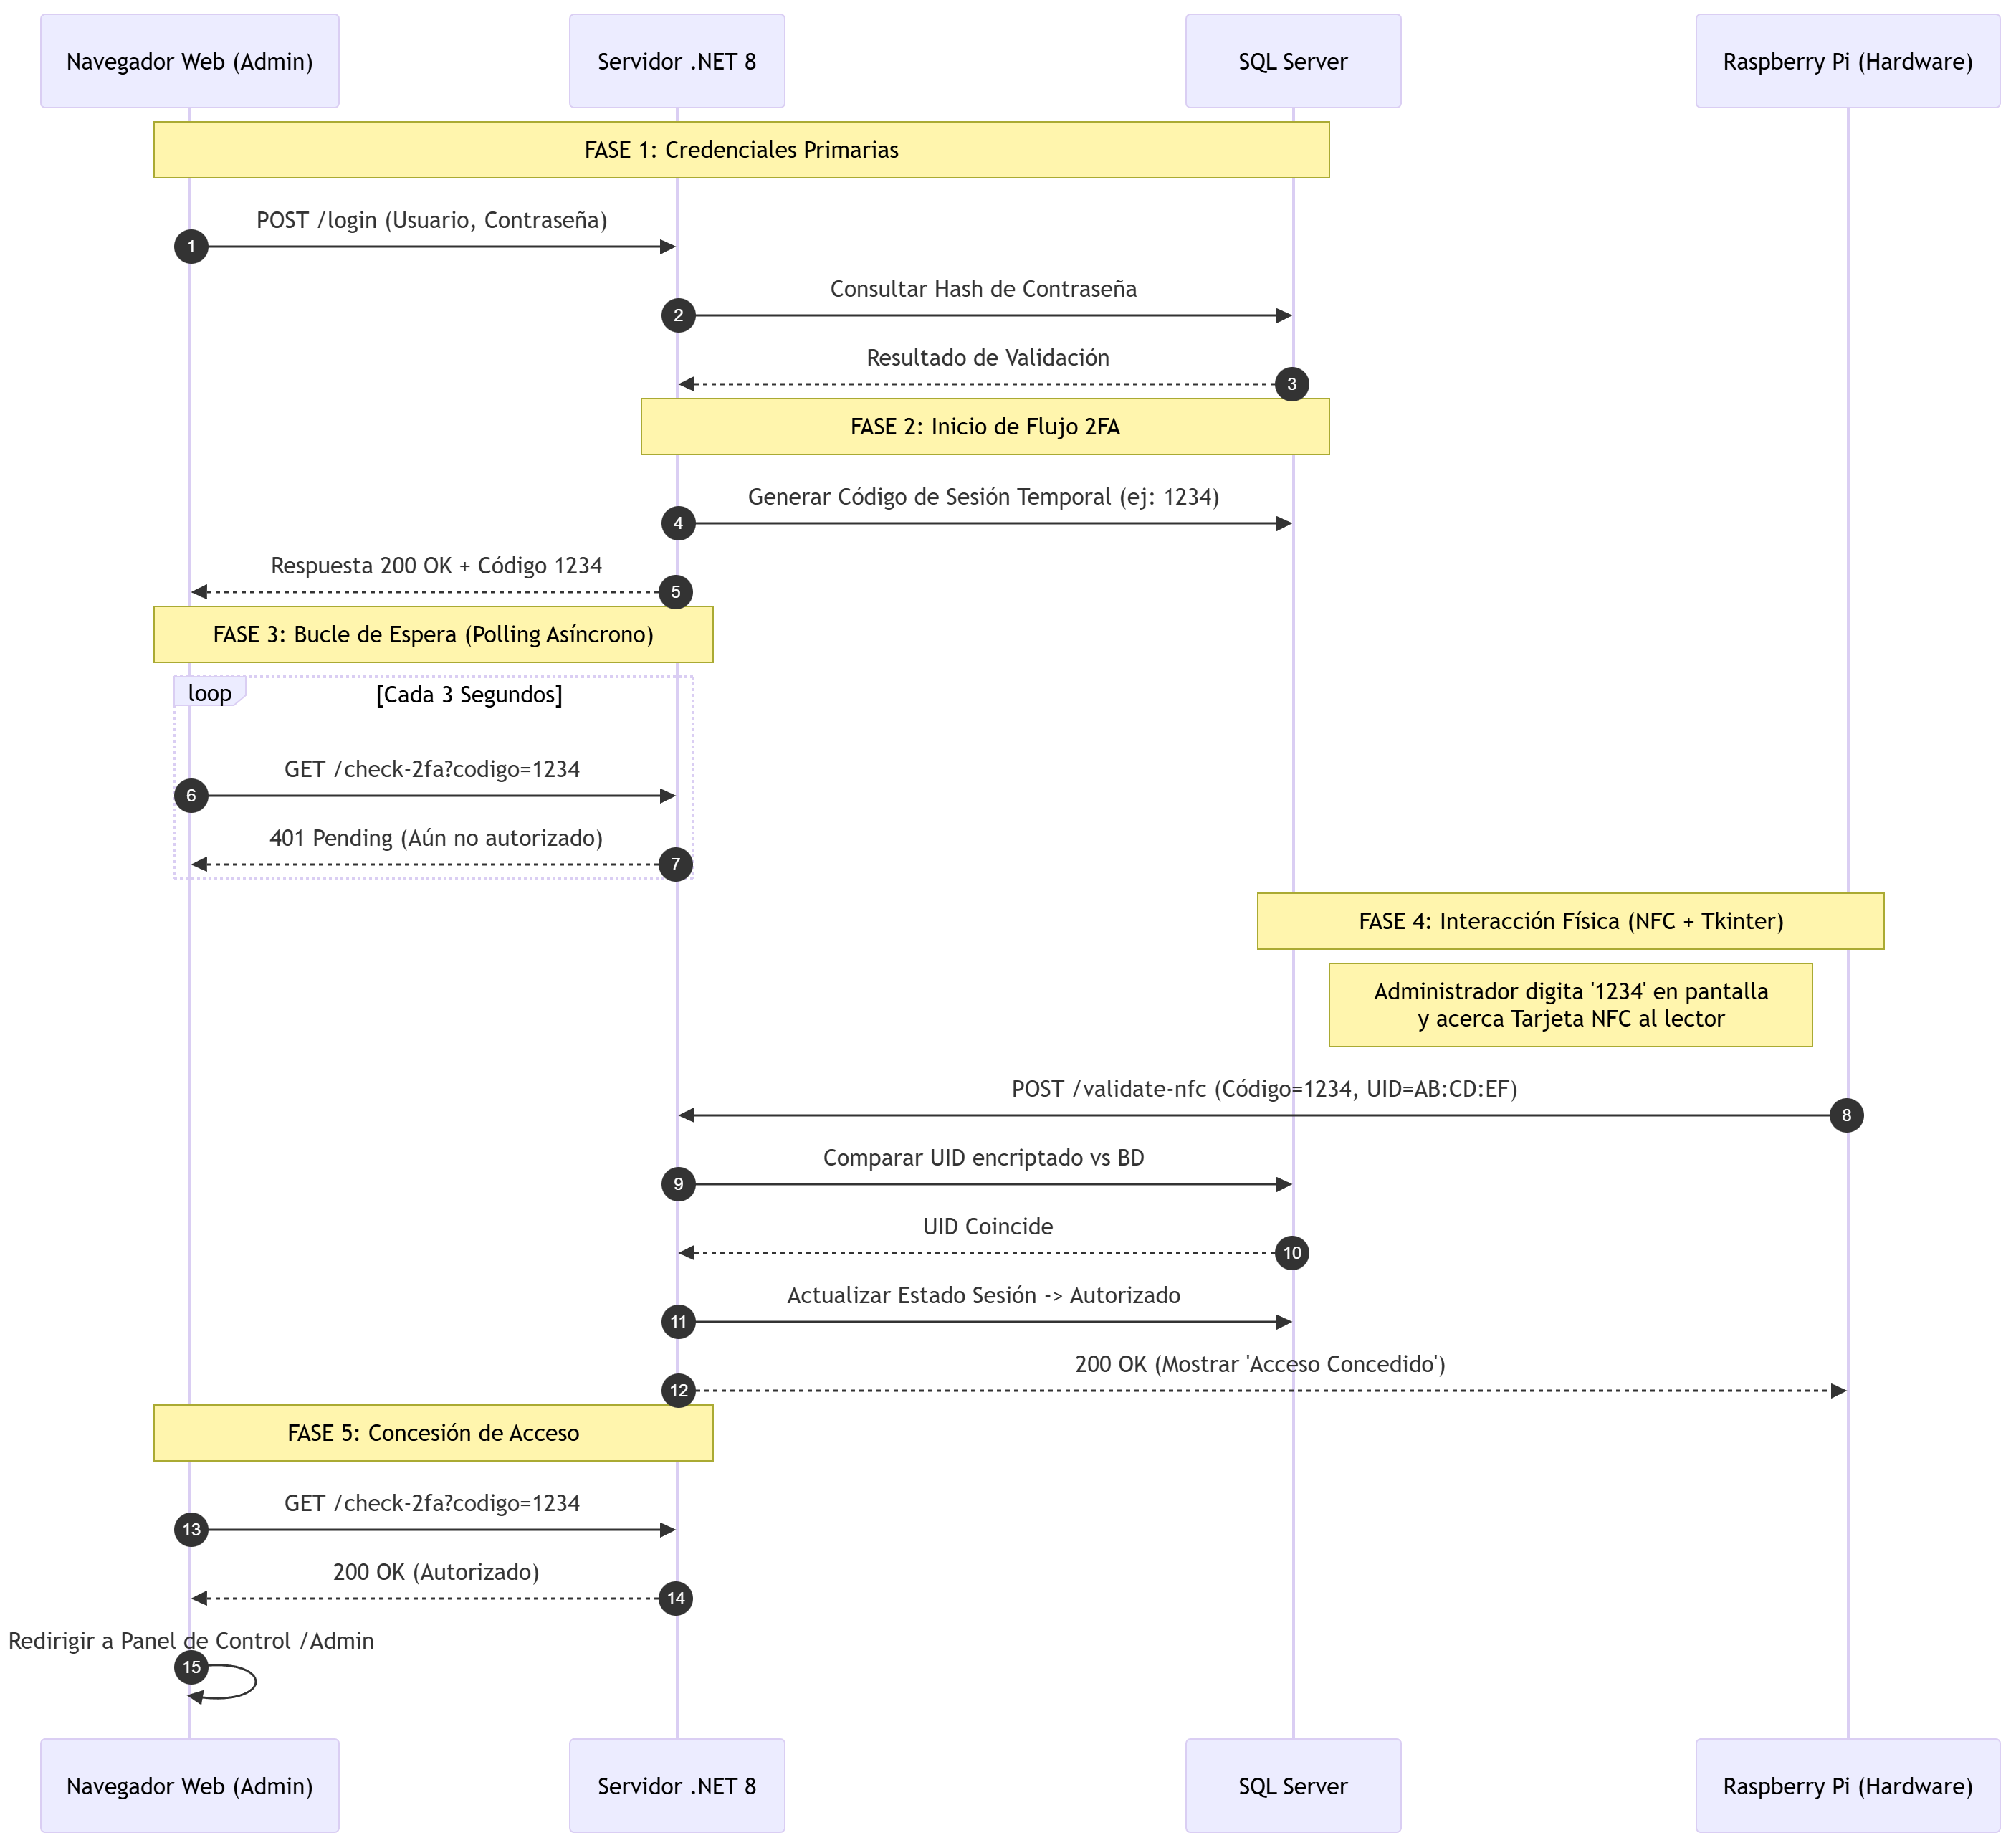
\includegraphics[width=0.98\textwidth]{imagenes/diagrama_secuencia_2fa.png} 
	\caption{Diagrama de Secuencia UML detallando el proceso de autenticación de doble factor y comunicación con la API (Creado en Mermaid.live).}
	\label{fig:uml_secuencia_2fa}
\end{figure}


\subsection{Diseño e Integración Física del Módulo (Impresión 3D)}

Para asegurar la durabilidad del módulo en entornos comerciales, se desarrolló una carcasa personalizada que integra la Raspberry Pi, la pantalla táctil y el lector NFC en una unidad compacta y ergonómica. El modelado 3D se basó en un levantamiento dimensional preciso de los componentes para garantizar un ensamblaje libre de tensiones mecánicas en los puertos y conexiones GPIO.

Una consideración técnica clave fue la ubicación del módulo RFID-RC522. El soporte interno fija el sensor de forma que su antena permanezca paralela a la cara interna del chasis. Dado que los polímeros de impresión no bloquean las señales de 13.56 MHz, la lectura de tarjetas es efectiva a través del material. Este diseño mantiene la electrónica sellada y protegida contra derrames de líquidos o suciedad, riesgos críticos en la operación de un restaurante.

La materialización se realizó mediante impresión 3D por deposición de hilo fundido (FDM). La Figura \ref{fig:carcasa} muestra el modelo digital diseñado y la Figura \ref{fig:carcasa_render} presenta el ensamblaje final, consolidando los componentes individuales en un dispositivo operativo tipo appliance.

% Opción A: Imágenes una debajo de la otra
\begin{figure}[H]
	\centering
	\includegraphics[width=0.8\textwidth]{imagenes/carcasa.png} 
	\caption{Modelado 3D de la carcasa protectora (Creado en Cinema 4D Trial Version)}
	\label{fig:carcasa}
\end{figure}

\begin{figure}[H]
	\centering
	\includegraphics[width=0.8\textwidth]{imagenes/carcasa_mult.png} 
	\caption{Modelado 3D de la carcasa protectora (Creado en Cinema 4D Trial Version)}
	\label{fig:carcasa_render}
\end{figure}

%%%%%%%%%%%

\section{Pruebas de Validación y Verificación}
En estricto cumplimiento con el diseño metodológico trazado en la fase de formulación del proyecto, la etapa de pruebas de validación y verificación se estructuró con el propósito de evaluar la funcionalidad, el rendimiento y la seguridad del sistema en un entorno que simulara fielmente las limitaciones tecnológicas reales de un restaurante PYME. 

Para abarcar integralmente el comportamiento del software, el plan de pruebas se dividió en cuatro frentes de evaluación: validación manual de usabilidad, pruebas unitarias de seguridad y lógica de negocio, pruebas automatizadas de estrés, y medición de latencia operativa.

\subsection{Infraestructura y Entorno de Laboratorio}
Para garantizar que el desempeño de la aplicación corresponda a la realidad económica de los establecimientos objetivo, la infraestructura del servidor principal —encargada de procesar la lógica de negocio en .NET 8 y gestionar la persistencia en la base de datos SQL Server— se desplegó de manera deliberada en un equipo con recursos heredados. Se utilizó un computador portátil DELL (año de fabricación 2008), equipado con un procesador Intel Core 2 Duo (T8000), 8 GB de memoria RAM DDR2 y un disco duro mecánico (HDD). Para maximizar la asignación de recursos hacia el sistema web, este equipo operó bajo el sistema operativo Windows 10 LTSC (Long-Term Servicing Channel).

La red de intranet fue gestionada mediante un router doméstico ZTE ZXV10 W300, operando estrictamente en modo local sin salida a internet. Para replicar la topología de red de un restaurante y evaluar el impacto de las conexiones mixtas, los clientes que simularon los módulos fijos (Cocina y Caja) fueron conectados mediante cableado a los puertos LAN. En contraste, el equipo encargado de simular al Mesero se enlazó exclusivamente a través de la interfaz inalámbrica en la banda Wi-Fi de 2.4 GHz. Esta distinción física resultó fundamental para introducir latencia real, susceptibilidad a interferencias y fluctuaciones de red, emulando el comportamiento de un dispositivo móvil operado en constante movimiento. Debido a requerimientos de compatibilidad del entorno de automatización, los clientes de prueba operaron bajo el sistema operativo Ubuntu.

\subsection{Verificación Manual de Funcionalidades}
Esta etapa consistió en una auditoría de completitud del software mediante pruebas manuales controladas. El propósito fue confirmar que la arquitectura final del sistema no omitiera ninguna de las herramientas operativas requeridas por los diferentes roles de usuario, garantizando la usabilidad de las interfaces gráficas.

Mediante una lista de verificación (\textit{Checklist}) trazada desde la matriz de requerimientos, se inspeccionaron los módulos de la plataforma:
\begin{itemize}
	\item \textbf{Módulo de Administrador:} Gestión de menú, reportes de ventas y administración de perfiles de empleados.
	\item \textbf{Módulo de Mesero:} Interfaz táctil para la toma ágil de pedidos, envío de comandas y visualización del estado de las mesas.
	\item \textbf{Módulo de Cocina:} Recepción en tiempo real de órdenes estructuradas y actualización del estado de preparación de los platos.
	\item \textbf{Módulo de Caja:} Acceso al resumen de cuentas por mesa, facturación y generación del cierre de servicio.
\end{itemize}

\subsection{Pruebas Unitarias y de Seguridad Lógica}
Para certificar la robustez interna de la aplicación, especialmente en el manejo de datos sensibles y control de accesos, se incorporó una batería de pruebas a nivel de código utilizando el marco de pruebas \textit{MSTest} para .NET 8. 

A diferencia de las pruebas de interfaz, estas evaluaciones se enfocaron en validar de forma aislada la lógica de negocio y los componentes de seguridad implementados en el \textit{backend}. Los escenarios evaluados incluyeron:
\begin{itemize}
	\item \textbf{Cifrado e Integridad:} Validación de los algoritmos de encriptación de credenciales en la base de datos, asegurando que no existan vulnerabilidades de almacenamiento en texto plano.
	\item \textbf{Control de Autorización:} Verificación de los filtros de sesión, garantizando que un usuario con un rol inferior (ej. Mesero) no pueda ejecutar métodos HTTP restringidos a roles superiores (ej. Administrador).
	\item \textbf{Autenticación de Doble Factor (2FA):} Pruebas de integración sobre los servicios que procesan los identificadores criptográficos generados por las tarjetas NFC, validando su correcta asociación con los usuarios registrados en SQL Server a través de Entity Framework 6.
\end{itemize}

\subsection{Pruebas Automatizadas de Concurrencia}
Para superar las limitaciones de una prueba manual esporádica y garantizar la estabilidad del sistema ante cargas de trabajo prolongadas, la validación operativa se llevó a cabo utilizando scripts automatizados desarrollados en \textit{Playwright} con Node.js. 

Se estructuró un entorno de estrés donde agentes virtuales autónomos interactuaron de manera simultánea durante una jornada operativa simulada de 9 horas ininterrumpidas. El agente \textit{Mesero} generó ráfagas constantes de pedidos, mientras que los agentes de \textit{Cocina} y \textit{Caja} interceptaron y despacharon estas solicitudes. Los resultados de esta ejecución masiva fueron recolectados en registros tabulares (archivos CSV) para documentar la tasa de éxito transaccional. Este enfoque validó la capacidad de Entity Framework 6 para procesar múltiples peticiones simultáneas sin generar interbloqueos (\textit{deadlocks}) ni corrupción de información referencial.

\subsection{Evaluación del Tiempo de Respuesta Operativa}
En estricta correspondencia con el objetivo de erradicar los retrasos del modelo manual de toma de pedidos, se ejecutó la medición empírica de la latencia del sistema. El registro de tiempos se focalizó en las operaciones transaccionales más demandantes utilizando herramientas de diagnóstico (\textit{DevTools - Network}) y cronometría física:
\begin{itemize}
	\item El tiempo neto desde que el Mesero confirma una comanda hasta que es persistida en la base de datos y renderizada en la pantalla de Cocina.
	\item La latencia en la resolución de consultas financieras y de inventario complejas.
	\item El tiempo de procesamiento del hardware 2FA, abarcando desde el contacto de la tarjeta física con el lector RFID-RC522 en la Raspberry Pi, hasta que el cliente Python valida el identificador con la API .NET y el sistema web autoriza el inicio de sesión.
\end{itemize}

El criterio de aceptación ineludible dicta que, incluso operando sobre el hardware heredado evaluado, el tiempo de respuesta total para cualquiera de estas operaciones críticas no debe exceder el umbral máximo de \textbf{2.0 segundos}.
